\documentclass[document.tex]{subfiles}
\begin{document}
\section*{Exercise 2:}


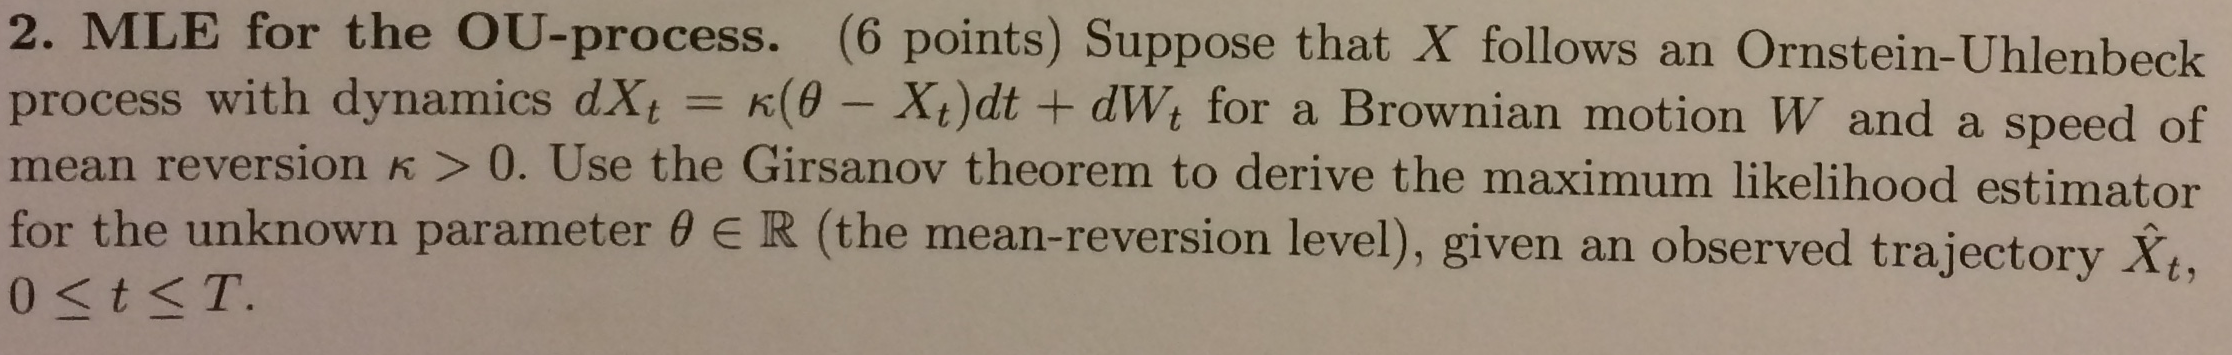
\includegraphics[width=\textwidth]{ex2.png}

The OU-process satisfies the following SDE:
\begin{equation}
dX_t = \kappa(\theta - X_t)dt + dW_t
\end{equation}

The distribution of $X_t$ is $P^{\mu}$ and depends on $\mu$. To find the MLE of $\theta$ we have to maximize the likelihood of our process $L(X;\mu)$. Suppose there is measure such that $P^{\mu} {\raise.17ex\hbox{$\scriptstyle\sim$}} \tilde{P}$ and
\begin{equation}
\frac{dP^{\mu}}{\tilde{P}} = L(X;\mu)
\end{equation}

We choose $\tilde{P}$ equal to the Wiener measure and we get:
\begin{equation}
\frac{dP^{\mu}}{\tilde{P}} = exp(\kappa (\theta - X_t)X_t - \frac{1}{2} \kappa^2(\theta - X_t)^2 t)
\end{equation}

To maximize the exponential is to maximize its argument. We derive w.r.t. $\theta$ and set equal to zero:
\begin{equation}
\kappa \hat{X}_t - \kappa^2(\theta - \hat{X}_t) t = 0
\end{equation}
\begin{equation}
\frac{ \hat{X}_t }{ \kappa } = \theta - \hat{X}_t
\end{equation}
\begin{equation}
\hat{\theta}_{MLE} = \frac{ \hat{X}_t }{ \kappa } + \hat{X}_t = \hat{X}_t (1 + \frac{ 1 }{ \kappa })
\end{equation}

\end{document}
